\chapter{实验与评测}
\sys 是一个高效的时序图处理系统,为了检验系统的性能,本文设计了一系列实验从多个角度对系统的性能进行全面的评测。
本章将对各实验的设计和结果进行详细的介绍,并给出各实验数据的详细分析。

\section{实验配置}
\noindent\textbf{实验环境}\ 系统运行在一个由8台机器组成的集群中,其中一台机器用作字符串服务器节点,一台机器运行分析节点,其余6台机器运行查询节点。每台机器都配备了两个Intel Xeon E5-2650 CPU,每个CPU都有8个核心、16个超线程。每台机器的内存都是128GB,都配备一张Mellanox
ConnectX-5 100Gbps InfiniBand网卡。8台机器通过一台Mellanox 100Gbps InfiniBand交换机互联。
所有机器运行的操作系统都是Ubuntu 16.04 (4.15.0-46-generic),InfiniBand网卡驱动为MLNX\_OFED\_LINUX-4.9-3.1.5.0。
其他软件版本为gcc/g++ v7.4.0、cmake v3.22.0和Python v3.8。

\noindent\textbf{使用的数据集}\ 实验使用的RDF数据集是开源项目LUBM\cite{lubm}生成的数据集。LUBM是里海大学发布的用于评测RDF数据集管理系统的查询性能的基准测试项目,LUBM数据集描述了大学里各种实体之间的关系,例如学生、教师、学院和课程等。生成数据集时,可以通过指定数据集包含的大学的数量来设置生成的数据集的规模,实验使用的数据集是LUBM 10240,它包含337M个实体,1410M个三元组。
LUBM数据集本身不包含时序数据,我们为每个三元组都随机生成了两个64位INT型时间戳$t_1$和$t_2$($t_1<t_2$,时间戳是从1970-01-01T00:00:00Z开始经过的秒数),分别表示三元组有效时间区间的开始时间和截止时间,得到的时序数据集称为tLUBM 10240。

实验使用的时序超图数据集是一个现实的金融数据集FIN,它描述了金融领域中的上市公司、基金、客户和供应商等之间的关系,包含661K条时序超边和360K个顶点。

图存储结构\store 和\newstore 的微观性能评测使用了LDBC SNB\cite{snb}、Wiki\cite{wiki}、R-MAT\cite{rmat}、UK-2005\cite{uk}和Twitter-2010\cite{twitter}5个图数据集。
LDBC SNB是一个图分析系统的基准测试项目,它包含一个社交网络图数据集生成器和多种图分析工作负载。
LDBC SNB数据集是一个描述社交网络中人、论坛、帖子和评论等实体之间关系的图,在生成数据集时,可以通过指定规模因子 (scale factor, SF)来控制生成的数据集的大小,实验使用的数据集SF=10。Wiki、R-MAT、UK-2005和Twitter-2010都是现实的图数据集。5个图数据集的统计信息见表\ref{tab:dataset}。

时序图分析模块的事务处理性能和图分析性能评测使用的是LDBC SNB (SF=10)基准测试,数据集会通过数据生成器提前生成,所有顶点和50\%的边会被批量加载到系统中,剩余50\%的边会通过客户端发起的图更新事务插入到系统中。

\begin{table}[!hpt]
  \bicaption{LDBC SNB (SB)、Wiki (WK)、R-MAT (RM)、UK-2005 (UK)和Twitter-2010 (TW) 5个图数据集的统计信息}{Statistics of 5 graph datasets: LDBC SNB (SB), Wiki (WK), R-MAT (RM), UK-2005 (UK) and Twitter-2010 (TW)}
  \label{tab:dataset}
  \centering
  \begin{tabular}{p{2cm}p{1cm}p{1cm}p{1cm}p{1cm}p{1cm}} \toprule
    \textbf{图数据集}\centering & \textbf{SB} & \textbf{WK} & \textbf{RM} & \textbf{UK} & \textbf{TW} \\ \midrule
    |V|\centering & 7.5M & 5.7M & 5.0M & 39.5M & 41.7M \\
    |E|\centering & 8.8M & 130M & 300M & 936M & 1.47B \\
    \bottomrule
  \end{tabular}
\end{table}

\noindent\textbf{实验基准}\
为了评测系统处理时序RDF图查询的性能,我们将\sys 与NebulaGraph和Neo4j两个系统进行了对比。
NebulaGraph和Neo4j都是基于属性图模型的图数据库,NebulaGraph支持分布式的存储和图查询处理,而Neo4j是单机图数据库。为了实现NebulaGraph和Neo4j对tLUBM 10240数据集的存储,我们将tLUBM 10240通过表\ref{tab:rdf2prop}中列出的映射转换为属性图数据集。NebulaGraph和Neo4j支持的图查询语言分别是nGQL和Cypher,SPARQL-T查询语句都可以转换成这两种查询语言。

\begin{table}[!hpt]
  \bicaption{时序RDF图到属性图的映射}{Mapping from temporal RDF graph to property graph}
  \label{tab:rdf2prop}
  \centering
  \begin{tabular}{p{8cm}p{7cm}} \toprule
    \textbf{时序RDF图} & \textbf{属性图} \\ \midrule
    时序三元组中的主语和宾语(表示类型名的宾语除外) & 顶点名 \\
    表示类型名的宾语 & 顶点类型 \\
    时序三元组中的主语、谓词和宾语(描述主语类型的时序三元组除外) & 主语对应的顶点指向宾语对应的顶点的有向边,边的类型是谓词 \\
    时序三元组中的有效时间区间(描述主语类型的时序三元组除外) & 对应边的两个属性 \\
    描述主语类型的时序三元组的有效时间区间 & 主语对应的顶点的两个属性 \\
    \bottomrule
  \end{tabular}
\end{table}

由于超图查询系统相关研究工作很少,所以我们并没有找到合适的基准时序超图查询系统来与\sys 作对比,我们的方案是将与时序超图数据集FIN等价的时序RDF图数据集加载到\sys 的时序RDF图存储中,然后通过等价的HQL-T和SPARQL-T查询语句来对比在查询等价数据时,\sys 的时序超图查询的性能和时序RDF图查询的性能。将时序超图数据集转换为时序RDF图数据集的方法为:将类型为\texttt{ty}、名称为\texttt{name}、连接$n$个顶点$v_1,v_2,...,v_n$、有效时间区间为$[t_1,t_2)$的时序超边转换为$n$个时序三元组$\{(\texttt{name} \ \texttt{ty} \ v_i \ [t_1, t_2))\ | \ 1\leq i \leq n,i\in Z\}$,将类型为\texttt{ty}、名称为\texttt{name}的顶点转化为时序三元组\texttt{name rdf:type ty [-$\infty$,+$\infty$)}。

为了对图存储结构\store 和\newstore 进行微观性能评测,我们选取了两种基准图存储结构CSR和LiveGraph的存储结构来进行比较。
LiveGraph的存储结构使用了高度优化过的邻接列表格式来存储图拓扑和属性数据,同时它使用的是一种细粒度的MVCC机制。
我们使用GraphScope\cite{gs}、Neo4j和LiveGraph三个支持图分析的基准系统来与\sys 的图事务处理性能和图分析性能进行对比。
GraphScope是一个先进的高性能离线图分析系统,由于它不支持图更新,所以我们会将图事务数据定期加载到其中。Neo4j虽然是一个图数据库,但它的图数据科学 (Graph Data Science, GDS)库实现了在图的最新快照上的图分析。这些系统上运行了三类图分析工作负载:

\begin{itemize}
    \item 三个常用图分析算法:网页排序 (PageRank, PR)、强连通分量 (Strong Connected Components, SCC) 和单源最短路径 (Single Source Shortest Path, SSSP);
    \item LDBC SNB提供的一个交互式查询IS-3和两个商业智能查询BI-2和BI-3;
    \item 三个图神经网络模型:GCN \cite{gcn}(Graph Convolution Network)、GSG\cite{gsg} (GraphSage) 和SGC\cite{sgc} (Simple Graph Convolution)。
\end{itemize}

\section{时序RDF图查询性能}
本文首先使用tLUBM 10240数据集对\sys 和各基准系统(NebulaGraph和Neo4j)的单个时序RDF图查询处理性能进行对比测试。
NebulaGraph运行在6台机器上,而由于Neo4j是单机系统,受存储空间限制,它无法完全加载tLUBM 10240数据集,所以我们仅让它们加载全部数据的4\%。
实验使用了6条SPARQL-T查询语句Q1-Q6作为工作负载,其中Q1和Q2是小查询、Q3和Q4是大查询、Q5和Q6包含时序三元组时间范围模式。
表\ref{tab:trdfeval}给出了各系统执行这6条查询的时延情况。与NebulaGraph相比,\sys 处理各查询都有一个数量级以上的性能优势,尤其是对于包含时序三元组时间范围模式的查询(Q5和Q6),\sys 的性能领先更加明显。
\sys 的性能提升主要得益于\sys 围绕RDMA的一系列存储结构和查询引擎上的设计和对时间条件查询的特殊优化。即使Neo4j存储的数据规模只有\sys 的4\%,它也需要消耗数倍以上的时间来处理相同的图查询请求。

\begin{table}[!hpt]
  \bicaption{Q1-Q8执行时延(毫秒)对比}{Q1-Q8 execution latency (msec) comparison}
  \label{tab:trdfeval}
  \centering
  \begin{tabular}{crrrr} \toprule
    & \textbf{\sys} & \textbf{NebulaGraph} & \textbf{Neo4j} \\ \midrule
    \textbf{Q1} & \textbf{0.26} & 12.00 & 13.25 \\
    \textbf{Q2} & \textbf{0.31} & 26.86 & 4.79 \\
    \textbf{Q3} & \textbf{172.02} & 3729 & 272 \\
    \textbf{Q4} & \textbf{153.87} & 3910 & 198 \\
    \textbf{Q5} & \textbf{3.70} & 2791 & 245 \\
    \textbf{Q6} & \textbf{19.59} & 1977 & 203 \\
    \bottomrule
  \end{tabular}
\end{table}

本文又测试了\sys 的并发查询处理性能,在本实验中,为了模拟高并发场景,系统为每个查询节点都创建4个代理线程和16个工作线程,每个代理线程都会不断地将Q1交给工作线程执行,代理线程会统计Q1的执行时延分布。图\ref{trdfcdf}是Q1的执行时延的累积分布函数(CDF),在高并发场景下,Q1的执行时延平均是执行单个Q1的8倍左右,P99尾时延也在10毫秒以内,这说明\sys 的FIFO查询请求执行模式可以使得其在高并发的场景下仍能保证每条查询请求的执行时延不至于过大。

\begin{figure}[!htb]
\center{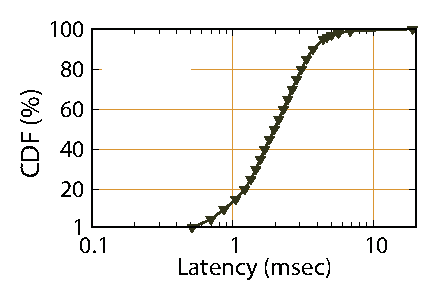
\includegraphics[width=0.4\textwidth]  {figures/cdf.eps}}
\bicaption{Q1执行时延的CDF}{The CDF of latency for Q1}
\label{trdfcdf}
\end{figure}

最后,本文从以下两个角度来测评\sys 处理时序RDF图查询的可扩展性:
\begin{itemize}
    \item 通过设置每个(共6个)查询节点上不同的工作线程数量,来研究系统的多线程可扩展性;
    \item 通过设置不同的查询节点数量,来研究系统的多机可扩展性。
\end{itemize}

\begin{figure}[!hpt]
\centering
\begin{minipage}{.45\linewidth}
\centering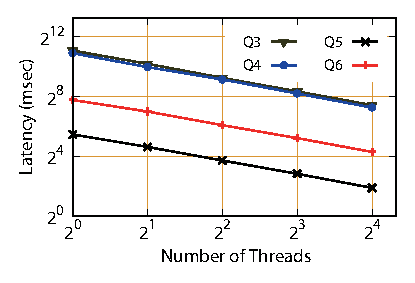
\includegraphics{figures/scale-thread1.eps}
\end{minipage}
\begin{minipage}{.45\linewidth}
\centering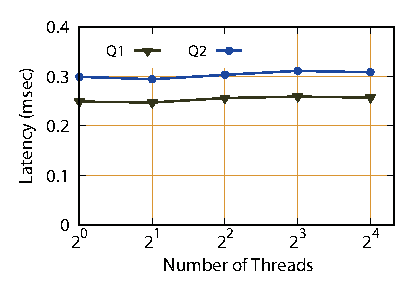
\includegraphics{figures/scale-thread2.eps}
\end{minipage} \\[10pt]
\begin{minipage}{1\linewidth}
\bicaption{不同工作线程时Q1-Q6的执行时延}{The latency of Q1-Q6 with different worker threads}
\label{scale-thread}
\end{minipage} \\[-10pt]
\end{figure}

图\ref{scale-thread}展示了Q1-Q6的执行时延与工作线程数量的关系,工作线程数量的增加能够给Q3-Q6带来接近线性的性能提升,而对Q1和Q2的执行时延几乎没有影响。这是因为Q3-Q6属于大查询,查询引擎会使用fork-join机制来处理这些查询,随着工作线程数量的增加,增加的工作线程会参与请求的执行;而Q1和Q2是小查询,系统只会使用一个工作线程来处理这两条查询,所以它们的执行时延和工作线程数量几乎是无关的。

\begin{figure}[!hpt]
\centering
\begin{minipage}{.45\linewidth}
\centering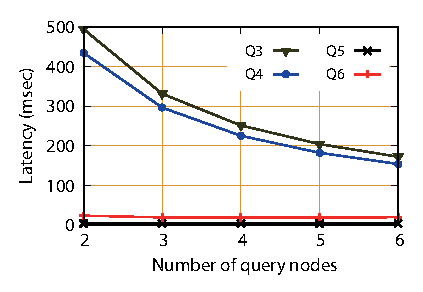
\includegraphics{figures/scale-server1.eps}
\end{minipage}
\begin{minipage}{.45\linewidth}
\centering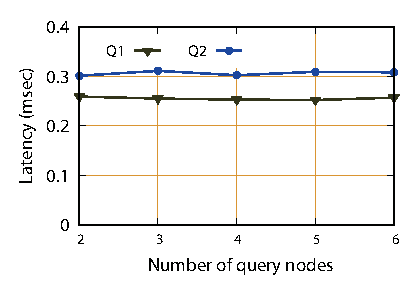
\includegraphics{figures/scale-server2.eps}
\end{minipage} \\[10pt]
\begin{minipage}{1\linewidth}
\bicaption{不同查询节点时Q1-Q6的执行时延}{The latency of Q1-Q6 with different query nodes}
\label{scale-server}
\end{minipage} \\[-10pt]
\end{figure}

图\ref{scale-server}是Q1-Q6在不同查询节点配置下的执行时延,Q3和Q4都是不包含时序三元组时间范围模式的大查询,查询节点数量的增加能够给这类查询带来接近线性的性能提升。查询节点数量的增加给Q4和Q5带来的性能提升不明显,原因是“时序三元组存储1”是按块划分到各查询节点上的,只有少数查询节点会存储符合查询指定时间条件的时序三元组。查询节点数量对Q1和Q2这类小查询的性能几乎没有影响。

\section{时序超图查询性能}
为了评测\sys 的时序超图查询的处理性能,本文首先构造了只包含单个SP的基础HQL-T查询Q1-Q7,由于FIN数据集中的顶点没有类型,所以我们没有构造GV查询。表\ref{tab:single}给出了这些查询的基本信息及\sys 处理这些基础查询和与它们等价的SPARQL-T查询的时延对比。
对于这些基础查询,\sys 都能达到亚毫秒级的执行时延。对于有些类型的SP(例如containEdges和inEdges等),HQL-T的查询效率更高,而有些类型的SP更适合转换为等价的SPARQL-T语句来执行,这些性能上的差异与数据集的特征有关。
与时序RDF图模型相比,时序超图模型更适合用来解决与集合关系有关的查询,因为HQL-T主要是为集合关系查询设计的一种查询语言,而SPARQL-T则需要使用较为复杂的查询语句才能实现集合关系查询。

\begin{table}[!hpt]
  \bicaption{\sys 处理HQL-T查询Q1-Q7和与它们等价的SPARQL-T查询的时延(微秒)对比}{Comparison of the latency (usec) of processing HQL-T queries Q1-Q7 and their equivalent SPARQL-T queries}
  \label{tab:single}
  \centering
  \begin{tabular}{cccc} \toprule
    & 类型 & HQL-T & SPARQL-T \\ \midrule
    \textbf{Q1} & etype & 1215 & 35 \\
    \textbf{Q2} & edges & 45 & 35 \\
    \textbf{Q3} & vertices & 46 & 34 \\
    \textbf{Q4} & intersectVertices & 93 & 182 \\
    \textbf{Q5} & intersectEdges & 237 & 150 \\
    \textbf{Q6} & containEdges & 81 & 285 \\
    \textbf{Q7} & inEdges & 65 & 148 \\
    \bottomrule
  \end{tabular}
\end{table}

最后,本文构造了一些包含多条模式的复杂HQL-T查询(Q8-Q14),表\ref{tab:multi}给出了这些查询语句的执行时延对比。

\begin{table}[!hpt]
  \bicaption{\sys 处理HQL-T查询Q8-Q14和与它们等价的SPARQL-T查询的时延(毫秒)对比}{Comparison of the latency (msec) of processing HQL-T queries Q8-Q14 and their equivalent SPARQL-T queries}
  \label{tab:multi}
  \centering
  \begin{tabular}{cccc} \toprule
    & HQL-T & SPARQL-T \\ \midrule
    \textbf{Q8} & 277.0 & 1266.8 \\
    \textbf{Q9} & 17.9 & 7.7 \\
    \textbf{Q10} & 8.7 & 1.0 \\
    \textbf{Q11} & 1147.1 & 1037.8 \\
    \textbf{Q12} & 268.7 & 499.9 \\
    \bottomrule
  \end{tabular}
\end{table}

\section{\store 和 \newstore 微观性能}
本节将对\store、\newstore、CSR和LiveGraph这四种图存储结构在内存使用、写吞吐量和读吞吐量等方面的微观性能进行比较。为了模拟不同的真实工作负载,我们分别使用以下两种模式来将相同的图数据加载到各存储结构里:
\begin{itemize}
    \item 顺序插入:按照边的起点的ID的顺序插入各边,这模拟的是批量加载图数据集的场景;
    \item 随机插入:以随机的顺序插入各边,这模拟的是图的事务化更新场景。
\end{itemize}

本文首先测试了各存储结构上的单版本扫边性能,单版本扫边不需要版本检查,只涉及对图拓扑的扫描。实验使用每秒扫描到的边的数量来作为各种图存储结构的扫边吞吐量。如图\ref{read1v},CSR作为最紧凑的、数据局部性最好的存储结构,是理论上扫边性能最好的。
顺序插入时,各种图存储结构在不同数据集上表现出的相对性能基本一致。
例如,与CSR相比,\store 扫描Wiki数据集的性能下降约为68\%,而LiveGraph的性能下降超过80\%,这主要得益于\store 的段迁移过程能够使得各顶点的边块位置更加接近,实现更好的数据局部性,从而可以更好地从CPU的预取机制受益。\newstore 的扫边吞吐量超过\store 的2倍,主要原因是\newstore 简化了边块中的边的数据结构(移除了两个时间戳)。
LiveGraph中各顶点的邻接列表在内存中的位置是互不相关的,而\store 会将ID相近的顶点的邻接列表通过一块段内存空间关联起来,这种设计带来的性能提升在随机插入场景下尤为明显:\store 的扫边吞吐可达LiveGraph的2\textasciitilde 5.9倍,原因是随机插入使得LiveGraph中各顶点的邻接列表在内存中的分布更加混乱,而\store 仍能实现良好的数据局部性。

\begin{figure}[!hpt]
\centering
\begin{minipage}{.45\linewidth}
\centering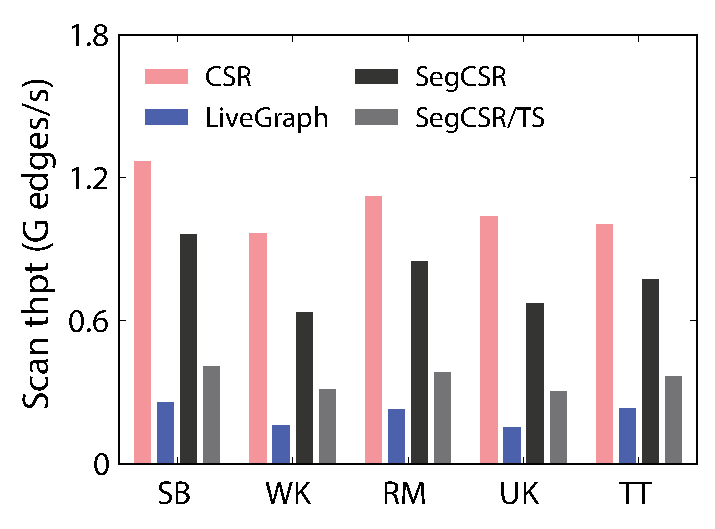
\includegraphics[scale=0.55]{figures/read-seq.eps}
\end{minipage}
\begin{minipage}{.45\linewidth}
\centering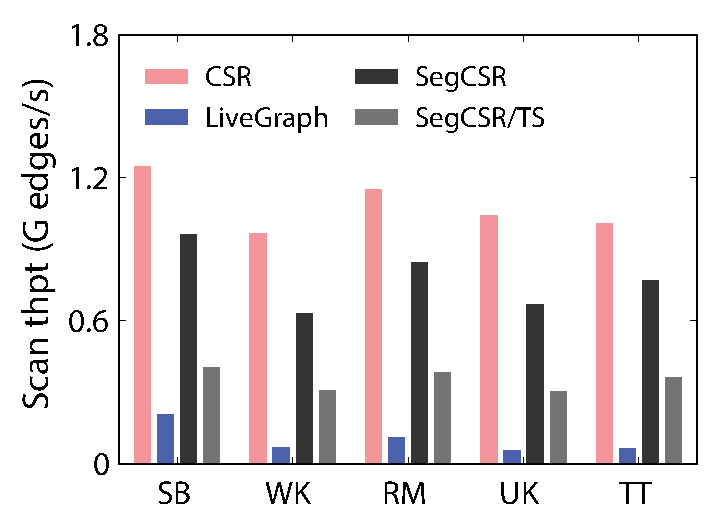
\includegraphics[scale=0.55]{figures/read-ran.eps}
\end{minipage} \\[10pt]
\begin{minipage}{1\linewidth}
\bicaption{顺序插入(左)和随机插入(右)时不同图存储结构扫边吞吐量的对比}{Comparison of edge scan throughput of different graph storage structures when sequential insertion (left) and random insertion (right)}
\label{read1v}
\end{minipage} \\[-10pt]
\end{figure}


图\ref{mem}给出了各种图存储结构的内存使用对比。
为了实现高效的图更新,\newstore 需要使用大约3倍于CSR的内存,但这比\store 和LiveGraph的要少得多。
粗粒度的MVCC机制使得\newstore 不用像\store 和LiveGraph一样为每条边都维护两个表示其生命周期的时间戳,只需要为每个顶点维护一个epoch表即可,这大大减少了时序数据的内存使用。由于段中存在空闲空间,SegCSR/TS的内存使用量比LiveGraph稍高,但通常多出不超过20\%。

\begin{figure}[!hpt]
\centering
\begin{minipage}{.45\linewidth}
\centering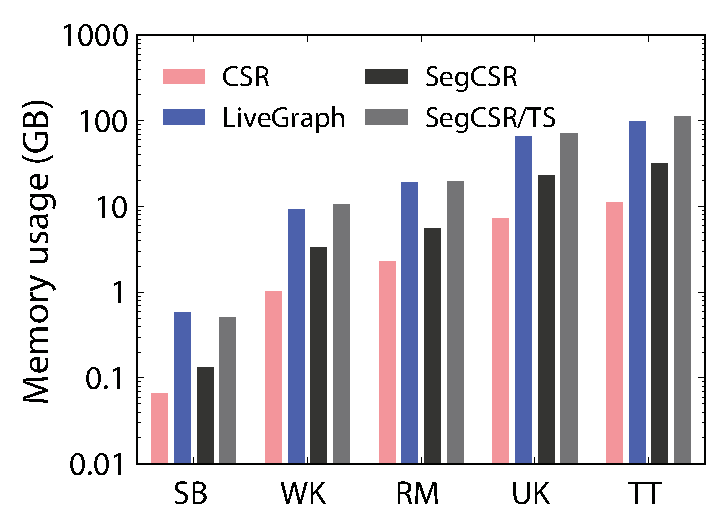
\includegraphics[scale=0.55]{figures/mem-seq.eps}
\end{minipage}
\begin{minipage}{.45\linewidth}
\centering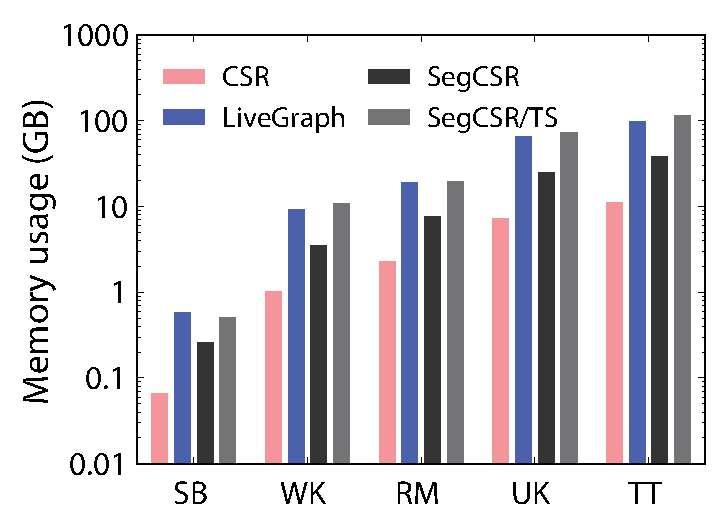
\includegraphics[scale=0.55]{figures/mem-ran.eps}
\end{minipage} \\[10pt]
\begin{minipage}{1\linewidth}
\bicaption{顺序插入(左)和随机插入(右)时不同图存储结构内存使用量的对比}{Comparison of memory usage of different graph storage structures when sequential insertion (left) and random insertion (right)}
\label{mem}
\end{minipage} \\[-10pt]
\end{figure}

图\ref{write}给出了各种图存储结构的写吞吐量对比,实验使用每秒插入边的数量来作为各种图存储结构的写吞吐量,由于CSR不支持更新,所以图中没有CSR的写吞吐量数据。
在顺序插入和随机插入两种情况下,\newstore 的写吞吐量分别为LiveGraph的2.2倍和2倍。
结合\store 的性能表现,\newstore 相对于LiveGraph的性能提升主要来源于粗粒度的MVCC机制:不需要为插入的每条边都写入版本号,只有在有新的版本(epoch)产生时才需要往边的起始顶点的epoch表中插入一个值。
性能提升的另一个来源是二者不同的垃圾回收机制:\newstore 的垃圾回收是由后台线程完成的,不在图更新操作的关键路径上,而LiveGraph的图更新操作则有可能触发在关键路径上的垃圾回收操作。
\newstore 的段迁移过程比较耗时,平均时延大约是普通插边操作的7000倍,这会导致图更新具有较高的尾延迟,但段迁移触发的频率较低(小于0.01\%)。

\begin{figure}[!hpt]
\centering
\begin{minipage}{.45\linewidth}
\centering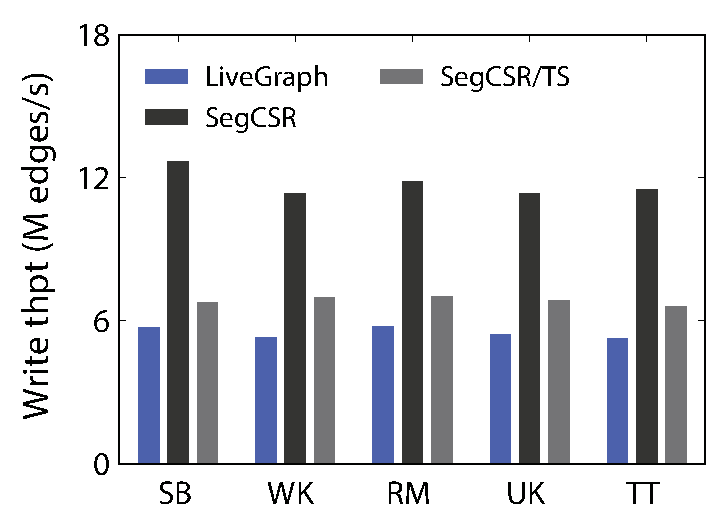
\includegraphics[scale=0.55]{figures/write-seq.eps}
\end{minipage}
\begin{minipage}{.45\linewidth}
\centering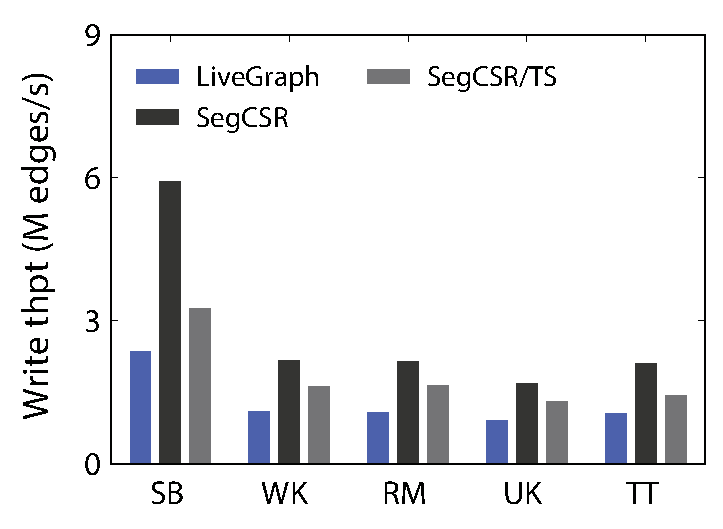
\includegraphics[scale=0.55]{figures/write-ran.eps}
\end{minipage} \\[10pt]
\begin{minipage}{1\linewidth}
\bicaption{顺序插入(左)和随机插入(右)时不同图存储结构写吞吐量的对比}{Comparison of write throughput of different graph storage structures when sequential insertion (left) and random insertion (right)}
\label{write}
\end{minipage} \\[-10pt]
\end{figure}

\section{图事务处理性能和图分析性能}
表\ref{tab:all}列出了GraphScope、Neo4j和LiveGraph三个支持图分析的基准系统与\sys 的图事务处理吞吐量和图分析时延的对比测试结果。

图事务处理方面,\sys 的性能领先LiveGraph约31\%,性能提升主要来源于\sys 使用的粗粒度的MVCC机制,它减少了\sys 在处理图事务时对时序数据的写入。Neo4j的图事务处理性能则是远远落后于\sys 和LiveGraph,原因可能是Neo4j对图的更新需要涉及复杂的索引更新操作。

图分析处理方面,GraphScope的图分析性能是最好的(除了IS-3,它是一个非常简单的图分析任务,16.9毫秒主要是GraphScope系统层面的开销),原因是它是一个离线图分析系统,使用了一种紧凑的图存储结构,且不需要版本数据的管理。\sys 的图分析性能是LiveGraph的1.4\textasciitilde 4.4倍,这些性能提升的主要来源是\newstore 基于段的边块管理策略和粗粒度的MVCC机制带来的数据访问量的下降和数据局部性的提升。Neo4j的图分析性能要远远落后于\sys,尤其是对于三个图分析算法PR、SCC和SSSP,二者的性能差距达到了一个数量级左右,原因是Neo4j的GDS库在执行这三个图分析算法时,会先把图的最新快照投影到内存中,然后在投影上执行图分析计算,投影过程消耗了大量时间。

\begin{table}[!hpt]
  \bicaption{\sys、GraphScope、Neo4j和LiveGraph的图事务处理吞吐量和图分析时延对比}{Comparison of graph transaction processing throughput and graph analysis latency of \sys, GraphScope, Neo4j and LiveGraph}
  \label{tab:all}
  \centering
  \begin{tabular}{crrrrr} \toprule
    & \textbf{\sys} & \textbf{GraphScope} & \textbf{Neo4j} & \textbf{LiveGraph} \\ \midrule
    \textbf{图事务} & 279K & $\times$ & 3.5K & 213K \\
    \hline
    \textbf{PR} & 377 & 309 & 5323 & 1276 \\
    \textbf{SCC} & 362 & 312 & 4726 & 1137 \\
    \textbf{SSSP} & 513 & 433 & 4668 & 1381 \\
    \hline
    \textbf{IS-3} & 0.0012 & 16.9 & 2.0 & 0.0039 \\
    \textbf{BI-2} & 235 & 201 & 568 & 828 \\
    \textbf{BI-3} & 292 & 266 & 573 & 1278 \\
    \hline
    \textbf{GCN} & 1097 & 940 & $\times$ & 1834 \\
    \textbf{GSG} & 1774 & 1443 & $\times$ & 2502 \\
    \textbf{SGC} & 779 & 717 & $\times$ & 1237 \\
    \bottomrule
  \end{tabular}
\end{table}

\section{本章小结}
本章对\sys 的性能进行了全面的评测。时序RDF图查询方面,系统的查询执行时延和基准系统NebulaGraph和Neo4j相比都能取得大幅度的性能领先;对于大查询,系统能够实现优秀的多线程可扩展性和多机可扩展性;在高并发场景下,系统也能够保证较低的平均执行时延和尾时延。时序超图查询方面,系统能够实现基础查询的亚毫秒级执行时延;系统处理时序超图和时序RDF图查询的性能接近,具体为图数据选择何种图模型取决于实际工作负载。图分析方面,微观性能评测实验表明,\newstore 能够通过更少的内存使用量,实现更高的读、写吞吐量(与LiveGraph相比);\sys 具有优秀的图事务处理性能和图分析性能。